% figure_b.tex — Dumbbell plot: Certain vs Uncertain flip rates (MMLU-Pro)
\documentclass[border=8pt]{standalone}
\usepackage[T1]{fontenc}
\usepackage{tikz}
\usepackage{pgfplots}
\pgfplotsset{compat=1.18}

% ── Colours ──────────────────────────────────────────────────────────
\definecolor{teal}{RGB}{13,148,136}
\definecolor{coral}{RGB}{225,29,72}
\definecolor{slate}{RGB}{55,65,81}
\definecolor{lightgray}{RGB}{156,163,175}
\definecolor{midgray}{RGB}{107,114,128}

\begin{document}
\sffamily
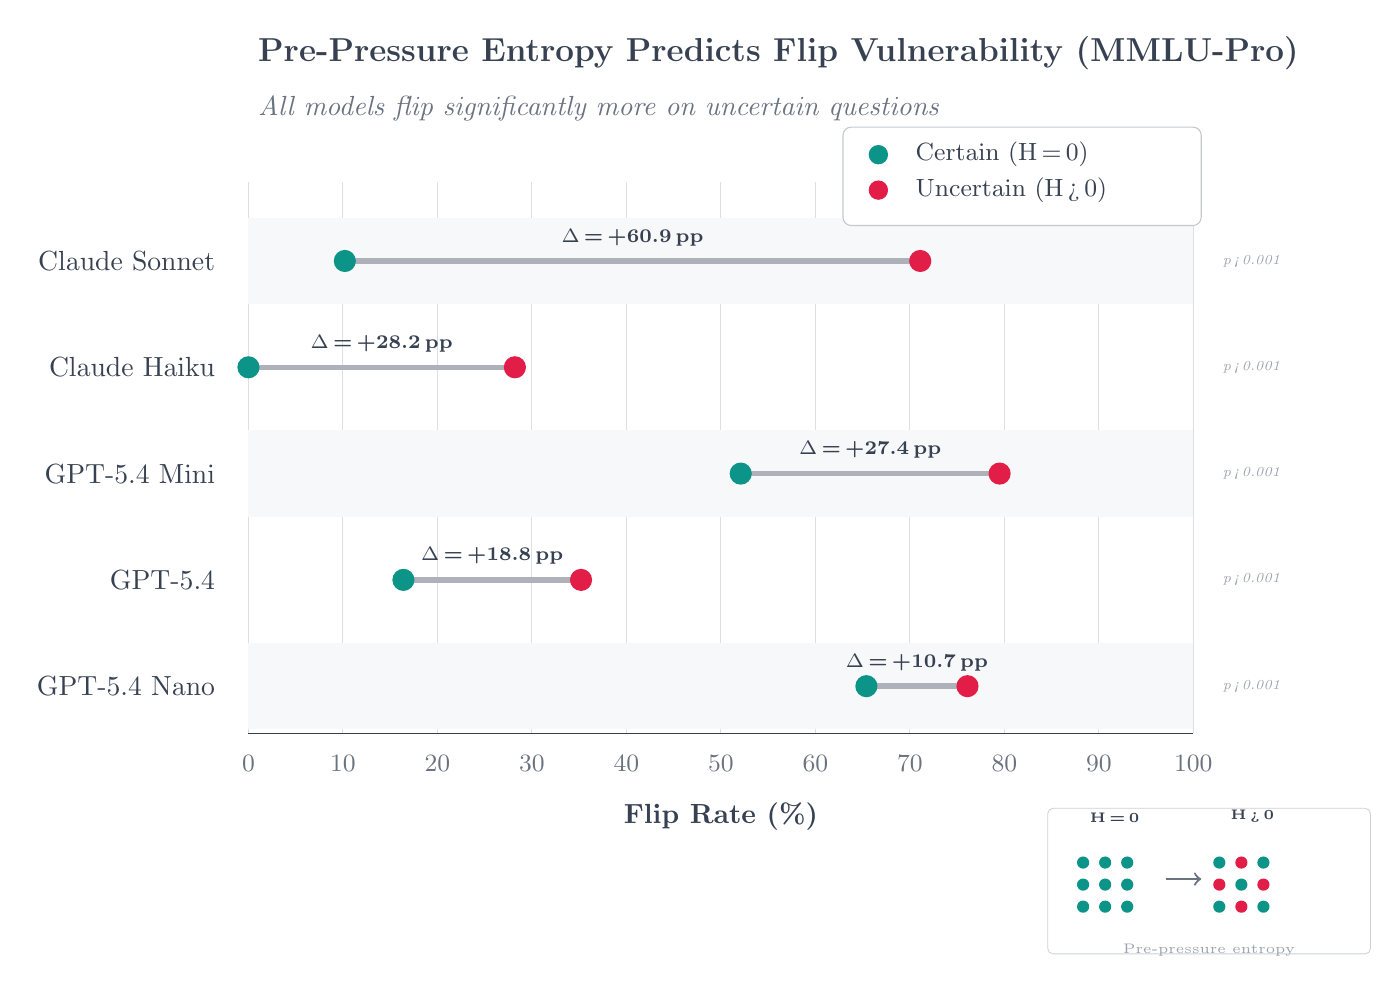
\begin{tikzpicture}

% ── Dimensions ───────────────────────────────────────────────────────
\def\plotW{12}     % width of the plot area in cm
\def\plotH{7.0}    % height of the plot area in cm
\def\xmin{0}
\def\xmax{100}
\def\leftmargin{3.4}
\def\rightpad{1.8}  % extra space to the right for p-values

% ── Helper: map data value to x-coordinate ───────────────────────────
\pgfmathsetmacro{\xscale}{\plotW/(\xmax-\xmin)}

% ── Title & subtitle ────────────────────────────────────────────────
\node[anchor=south west, font=\bfseries\large, text=slate]
  at (\leftmargin, \plotH+1.3)
  {Pre-Pressure Entropy Predicts Flip Vulnerability (MMLU-Pro)};
\node[anchor=south west, font=\itshape\normalsize, text=midgray]
  at (\leftmargin, \plotH+0.65)
  {All models flip significantly more on uncertain questions};

% ── X-axis gridlines & labels ────────────────────────────────────────
\foreach \v in {0,10,20,30,40,50,60,70,80,90,100} {
  \pgfmathsetmacro{\xpos}{\leftmargin + (\v-\xmin)*\xscale}
  % gridline
  \draw[lightgray!35, thin] (\xpos, 0) -- (\xpos, \plotH);
  % tick label
  \node[anchor=north, font=\small, text=midgray] at (\xpos, -0.15) {\v};
}
% X-axis title
\node[anchor=north, font=\normalsize\bfseries, text=slate]
  at (\leftmargin + \plotW/2, -0.75) {Flip Rate (\%)};

% ── Data ─────────────────────────────────────────────────────────────
% Sorted by Δ descending (top to bottom):
% Row 4 (top):   Claude Sonnet   10.2   71.1   +60.9
% Row 3:         Claude Haiku     0.0   28.2   +28.2
% Row 2:         GPT-5.4 Mini    52.1   79.5   +27.4
% Row 1:         GPT-5.4         16.4   35.2   +18.8
% Row 0 (bot):   GPT-5.4 Nano   65.4   76.1   +10.7

\def\rowsep{1.35}  % vertical spacing between rows

% ── Macro to draw one row ────────────────────────────────────────────
% #1=row index, #2=model name, #3=certain%, #4=uncertain%, #5=delta string
\newcommand{\dumbbellrow}[5]{%
  \pgfmathsetmacro{\ypos}{0.6 + #1*\rowsep}%
  \pgfmathsetmacro{\xA}{\leftmargin + (#3-\xmin)*\xscale}%
  \pgfmathsetmacro{\xB}{\leftmargin + (#4-\xmin)*\xscale}%
  \pgfmathsetmacro{\xmid}{(\xA+\xB)/2}%
  % model label
  \node[anchor=east, font=\normalsize, text=slate] at (\leftmargin - 0.3, \ypos) {#2};
  % faint row stripe (alternating)
  \pgfmathparse{mod(#1,2)==0 ? 1 : 0}
  \ifnum\pgfmathresult=1
    \fill[lightgray!8] (\leftmargin, \ypos-0.55) rectangle (\leftmargin+\plotW, \ypos+0.55);
  \fi
  % connecting line
  \draw[midgray!55, line width=2pt, line cap=round] (\xA, \ypos) -- (\xB, \ypos);
  % teal dot (certain)
  \fill[teal] (\xA, \ypos) circle (4pt);
  % coral dot (uncertain)
  \fill[coral] (\xB, \ypos) circle (4pt);
  % delta annotation — single line
  \node[anchor=south, font=\scriptsize\bfseries, text=slate, inner sep=1pt]
    at (\xmid, \ypos+0.15) {$\Delta$\,=\,#5\,pp};
  % p-value annotation
  \node[anchor=west, font=\tiny, text=lightgray]
    at (\leftmargin + \plotW + 0.25, \ypos) {\textit{p\,<\,0.001}};
}

% ── Draw rows (bottom to top) ───────────────────────────────────────
\dumbbellrow{0}{GPT-5.4 Nano}{65.4}{76.1}{+10.7}
\dumbbellrow{1}{GPT-5.4}{16.4}{35.2}{+18.8}
\dumbbellrow{2}{GPT-5.4 Mini}{52.1}{79.5}{+27.4}
\dumbbellrow{3}{Claude Haiku}{0.0}{28.2}{+28.2}
\dumbbellrow{4}{Claude Sonnet}{10.2}{71.1}{+60.9}

% ── Bottom axis line ─────────────────────────────────────────────────
\draw[slate, thin] (\leftmargin, 0) -- (\leftmargin+\plotW, 0);

% ── Legend (upper-right) ────────────────────────────────────────────
\begin{scope}[shift={(\leftmargin+\plotW-4.2, \plotH-0.15)}]
  \fill[white, draw=lightgray!60, rounded corners=3pt, line width=0.4pt]
    (-0.25, -0.4) rectangle (4.3, 0.85);
  % Certain
  \fill[teal] (0.2, 0.5) circle (3.5pt);
  \node[anchor=west, font=\small, text=slate] at (0.55, 0.5) {Certain (H\,=\,0)};
  % Uncertain
  \fill[coral] (0.2, 0.05) circle (3.5pt);
  \node[anchor=west, font=\small, text=slate] at (0.55, 0.05) {Uncertain (H\,>\,0)};
\end{scope}

% ── Small inset: dot-grid concept (lower-right corner) ──────────────
\begin{scope}[shift={(\leftmargin+\plotW+\rightpad-3.2, -2.2)}]
  % background box
  \fill[white, draw=lightgray!50, rounded corners=2pt, line width=0.3pt]
    (-0.45, -0.6) rectangle (3.65, 1.25);

  % H=0 grid (all teal)
  \node[anchor=south, font=\tiny\bfseries, text=slate] at (0.4, 0.95) {H\,=\,0};
  \foreach \r in {0,1,2} {
    \foreach \c in {0,1,2} {
      \pgfmathsetmacro{\gx}{\c*0.28}
      \pgfmathsetmacro{\gy}{\r*0.28}
      \fill[teal] (\gx, \gy) circle (2.2pt);
    }
  }

  % arrow
  \draw[->, midgray, thick] (1.05, 0.35) -- (1.50, 0.35);

  % H>0 grid (mixed teal/coral)
  \node[anchor=south, font=\tiny\bfseries, text=slate] at (2.15, 0.95) {H\,>\,0};
  % Row 0
  \fill[teal]  (1.73, 0.0) circle (2.2pt);
  \fill[coral] (2.01, 0.0) circle (2.2pt);
  \fill[teal]  (2.29, 0.0) circle (2.2pt);
  % Row 1
  \fill[coral] (1.73, 0.28) circle (2.2pt);
  \fill[teal]  (2.01, 0.28) circle (2.2pt);
  \fill[coral] (2.29, 0.28) circle (2.2pt);
  % Row 2
  \fill[teal]  (1.73, 0.56) circle (2.2pt);
  \fill[coral] (2.01, 0.56) circle (2.2pt);
  \fill[teal]  (2.29, 0.56) circle (2.2pt);

  % tiny caption
  \node[anchor=north, font=\tiny, text=lightgray] at (1.6, -0.35)
    {Pre-pressure entropy};
\end{scope}

% ── Invisible anchor to ensure right padding ────────────────────────
\path (\leftmargin + \plotW + \rightpad, 0);

\end{tikzpicture}
\end{document}
